\chapter{Markdown ``flavours'', extensions, and their impacts}

\vspace{1cm}

Markdown achieved its objectives of readability and simplicity, which were the main arguments for its fast rise in popularity.
What started as a simple Perl script that converts Markdown to HTML via regex replacements became a phenomenon, and was adopted in many
famous online services and pieces of software.\newline

However, there is no real "specification" for Markdown beyond the original blog post introducing the language and a few other pages
on Gruber's website. With time, one of Markdown's strengths, it's simplicity, also became one of its flaws for a few reasons:

\begin{itemize}
    \item While integrating Markdown, many developers realised that unfortunately Markdown is filled with unintentional errors and breaking states, which generate invalid HTML.
    \item Lack of features
    \item Other output formats were often requested, chiefly PDF.
\end{itemize}

These qualities of Markdown outweighing the flaws, and opinionated people wanting to fix issues their own way, the proliferation of new syntaxes
and compilers that are supersets or modifications of the original syntax popped-up, which are commonly called "markdown flavours".

\section{One syntax, many implementations}

---

TODO:

Give context for figure below

---

\begin{figure}[h]
\centering
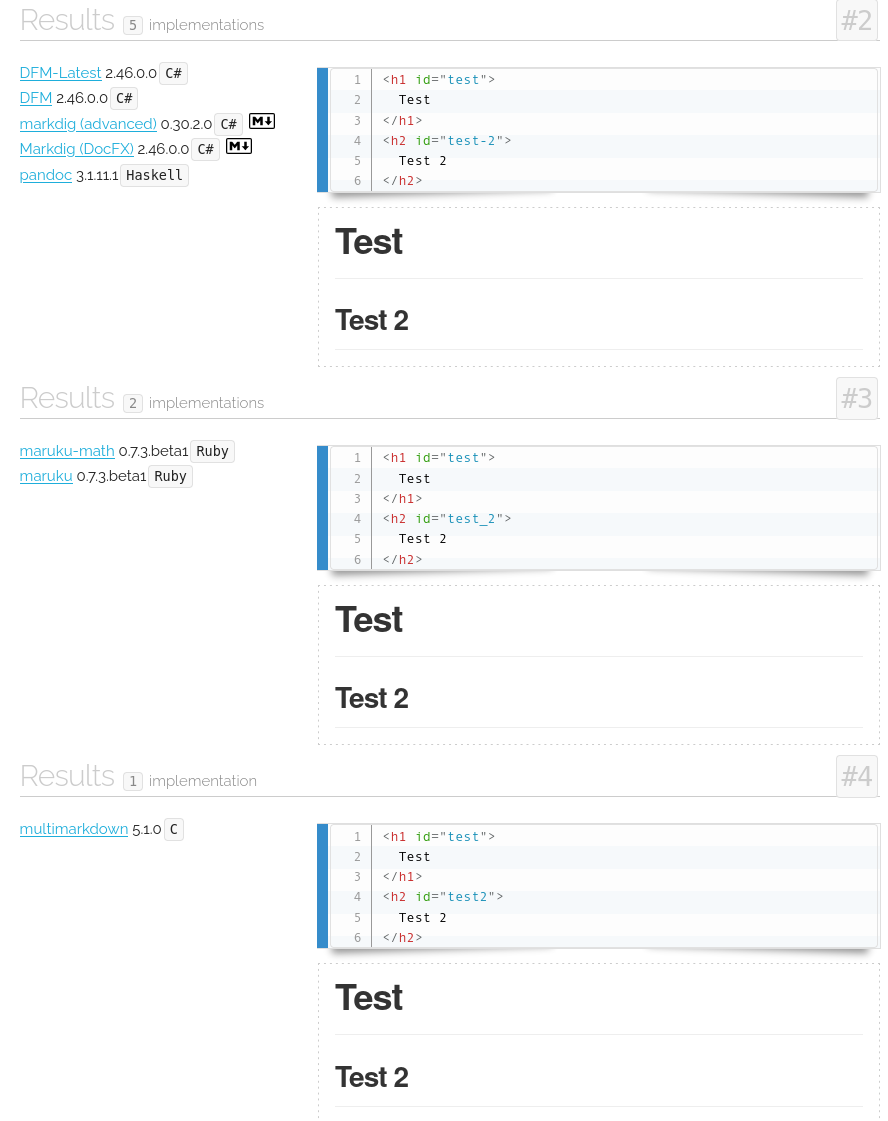
\includegraphics[scale=0.3]{babelmark}
\caption{Babelmark listing some of many possible outputs from markdown implementations}
\end{figure}

\section{Lack of features}

---

TODO:

List features missing and what approaches some implementations took

\begin{itemize}
    \item Limited formatting options
    \item Lack of tables and footnotes
    \item Lack of accessibility
    \item No support for Macros or Variables
    \item Lack of metadata
    \item GFM: task lists, tables, and syntax highlighting for code blocks
\end{itemize}

---

\section{Output formats}

---

TODO:

Discuss Pandoc, Github flavored markdown, etc

---